\chapter{Where Are the Genes?}
\label{ch:genes}

Genes are located on the DNA. :)

But where exactly? At this stage, let's define a gene as a specific region of the genome that contains a sequence of DNA which is transcribed into messenger RNA and subsequently translated into a protein.

By now, you may be familiar with the central dogma of molecular biology, which essentially explains the flow of genetic information: from DNA to RNA to protein. You also know that DNA is made up of two strands, and these strands run in opposite directions, meaning one strand is the reverse complement of the other. Genes can be found on either strand.

DNA and RNA are synthesized in the 5' to 3' direction. This means that during synthesis, a strand is read from 3' to 5' to create a complementary RNA strand. Consider an example fragment of the DNA:

\begin{verbatim}
    5'-TTT GGA TTC CGG-3'
    3'-AAA CCT AAG GCC-5'
\end{verbatim}

The fragment contains two strands: one running from 5' to 3' and the other running from 3' to 5'. Note that RNA can be synthesized from either of these two strands, and the RNA sequence will be the {\em reverse complement} of the DNA sequence. It will be a {\em complement} since the nucleotides pair with their complementary bases (A with U in RNA, T with A, G with C, and C with G), and reverse since the RNA strand is synthesized in the 5' to 3' direction, opposite to the template strand's 3' to 5' direction.

The {\em 5' to 3' strand} is often referred to as the {\em coding strand} (also known as the sense strand) because it has the same sequence as the mRNA, except that thymine is replaced with uracil in RNA. This is the strand that directly reflects the sequence of the resulting protein. The {\em 3' to 5' strand} is referred to as the {\em template strand} (also known as the antisense strand) because it serves as the template for RNA polymerase during transcription. RNA polymerase reads the template strand in the 3' to 5' direction to synthesize mRNA in the 5' to 3' direction.

In databases like {\em NCBI Nucleotide}, sequences are typically provided in the {\em 5' to 3' direction of the coding strand}. This means that the sequences listed usually correspond to the coding (sense) strand, which matches the mRNA sequence that would be produced (with thymine instead of uracil). Therefore, when we retrieve a nucleotide sequence from a database like NCBI, you are usually getting the sequence in the orientation of the coding strand, from the 5' to 3' end.

\section{Reading Frames}

A reading frame is a way of dividing a DNA or RNA sequence into consecutive, non-overlapping sets of three nucleotides, called codons, which correspond to amino acids during protein synthesis. Since each codon is three bases long, there are three possible reading frames for any given sequence, depending on where you start reading. The correct reading frame is crucial, as a shift in the frame can completely change the resulting amino acid sequence and therefore the function of the protein.

Consider again the DNA fragment we have seen before. If we read our sequence from left to right, the bottom strand is our template strand, and the top strand is our coding strand. Depending on which nucleotide we start with, the complementary nucleotides to the template strand are:

\begin{verbatim}
    TTT GGA TTC CGG
    TTG GAT TCG
    TGG ATT CCG
\end{verbatim}

Each sequence
\marginpar{\raggedright
Instead of thymine, the base used in RNA is uracil. We will leave the writing of the sequences as is. The coding tables are most often written in the DNA language.}
above represents the codons for that reading frame in DNA (not RNA), so thymine (T) is still shown instead of uracil (U). Notice also that instead of generating the reverse complement of the template strand, we can simply read the 5' to 3' strand directly, which is why it is called the coding strand, because its sequence already matches the mRNA (except that T replaces U). These three sequences would translate into three different sequences of amino acid sequences:
%
\begin{verbatim}
    Phe - Gly - Phe - Arg
    Leu - Asp - Ser
    Trp - Ile - Pro
\end{verbatim}

\begin{table}[!ht]
    \centering
    \small
    \begin{tabular}{|c|c|c|c|c|c|}
    \hline
    \multirow{2}{*}{1st Letter} & \multicolumn{4}{c|}{2nd Letter} & \multirow{2}{*}{3rd Letter} \\ \cline{2-5}
     & T & C & A & G &  \\ \hline
    T & \textbf{TTT} Phe & \textbf{TCT} Ser & \textbf{TAT} Tyr & \textbf{TGT} Cys & T \\
      & \textbf{TTC} Phe & \textbf{TCC} Ser & \textbf{TAC} Tyr & \textbf{TGC} Cys & C \\
      & \textbf{TTA} Leu & \textbf{TCA} Ser & \textbf{TAA} Stop & \textbf{TGA} Stop & A \\
      & \textbf{TTG} Leu & \textbf{TCG} Ser & \textbf{TAG} Stop & \textbf{TGG} Trp & G \\ \hline
    C & \textbf{CTT} Leu & \textbf{CCT} Pro & \textbf{CAT} His & \textbf{CGT} Arg & T \\
      & \textbf{CTC} Leu & \textbf{CCC} Pro & \textbf{CAC} His & \textbf{CGC} Arg & C \\
      & \textbf{CTA} Leu & \textbf{CCA} Pro & \textbf{CAA} Gln & \textbf{CGA} Arg & A \\
      & \textbf{CTG} Leu & \textbf{CCG} Pro & \textbf{CAG} Gln & \textbf{CGG} Arg & G \\ \hline
    A & \textbf{ATT} Ile & \textbf{ACT} Thr & \textbf{AAT} Asn & \textbf{AGT} Ser & T \\
      & \textbf{ATC} Ile & \textbf{ACC} Thr & \textbf{AAC} Asn & \textbf{AGC} Ser & C \\
      & \textbf{ATA} Ile & \textbf{ACA} Thr & \textbf{AAA} Lys & \textbf{AGA} Arg & A \\
      & \textbf{ATG} Met & \textbf{ACG} Thr & \textbf{AAG} Lys & \textbf{AGG} Arg & G \\ \hline
    G & \textbf{GTT} Val & \textbf{GCT} Ala & \textbf{GAT} Asp & \textbf{GGT} Gly & T \\
      & \textbf{GTC} Val & \textbf{GCC} Ala & \textbf{GAC} Asp & \textbf{GGC} Gly & C \\
      & \textbf{GTA} Val & \textbf{GCA} Ala & \textbf{GAA} Glu & \textbf{GGA} Gly & A \\
      & \textbf{GTG} Val & \textbf{GCG} Ala & \textbf{GAG} Glu & \textbf{GGG} Gly & G \\ \hline
    \end{tabular}
    \caption{Genetic code table.}
    \end{table}

We could also use the upper strain of the DNA fragment as the template strain. Let us write it in the 3' to 5' direction, that is, reading it from right to left:

\begin{verbatim}
    3'-GGC CTT AGG TTT-5'
\end{verbatim}

The complementary RNA strand would be:
\begin{verbatim}
    5'-CCG GAA TCC AAA-3'
\end{verbatim}

Using this strain, the three possible reading frames are:

\begin{verbatim}
    CCG GAA TCC AAA
    CGG AAT CCA
    GGA ATC CAA
\end{verbatim}

Which would translate into:

\begin{verbatim}
    Pro - Glu - Ser - Lys
    Arg - Asn - Pro
    Gly - Ile - Gln
\end{verbatim}

To read our DNA fragment,
\marginpar{\raggedright Given a DNA sequence and its reverse complement, we have six reading frames.}
we thus have six possibilities, three for each strain. And we thus get six different amino acid sequences. Let us automate this process using Python code, also to check if our transciptions and translations are correct.

\vspace*{3mm}
\begin{lstlisting}
from Bio.Seq import Seq
from Bio.Data import CodonTable

coding_seq = "TTTGGATTCCGG"

def reading_frame(seq, start):
    """Reading frame of a sequence starting at start position."""
    end = len(seq) - (len(seq[start:]) % 3)
    return seq[start:end]

def translate_reading_frames(seq):
    """Translate the reading frames of a sequence."""
    for i in range(3):
        frame = reading_frame(seq, i)
        rna_seq = Seq(frame).transcribe()
        protein_seq = rna_seq.translate(to_stop=True)
        print(f"Reading Frame {i + 1}:")
        print(f"Nucleotide sequence: {frame}")
        print(f"Amino acid sequence: {protein_seq}")
        print()

translate_reading_frames(coding_seq)
\end{lstlisting}

The code above will output the following:

\vspace*{3mm}
\begin{lstlisting}
Reading Frame 1:
Nucleotide sequence: TTTGGATTCCGG
Amino acid sequence: FGFR

Reading Frame 2:
Nucleotide sequence: TTGGATTCC
Amino acid sequence: LDS

Reading Frame 3:
Nucleotide sequence: TGGATTCCG
Amino acid sequence: WIP
\end{lstlisting}

Whcih is fine, but note that the aminoacids are here represented with single letters. To use the three-letter code, we need to add the following to our code (where appropriate):

\vspace*{3mm}
\begin{lstlisting}
aa_three_letter = {
    'A': 'Ala', 'R': 'Arg', 'N': 'Asn', 'D': 'Asp', 'C': 'Cys',
    'Q': 'Gln', 'E': 'Glu', 'G': 'Gly', 'H': 'His', 'I': 'Ile',
    'L': 'Leu', 'K': 'Lys', 'M': 'Met', 'F': 'Phe', 'P': 'Pro',
    'S': 'Ser', 'T': 'Thr', 'W': 'Trp', 'Y': 'Tyr', 'V': 'Val',
    '*': 'Stop'
}

def translate_to_three_letter(protein_seq):
    return "-".join(aa_three_letter[aa] for aa in protein_seq)

print(f"Final sequence: {translate_to_three_letter(protein_seq)}")
\end{lstlisting}

Let us change the code slightly, and output the translations for all the six reading frames. Notice that, given the coding sequence, we also need to translate all the frames from its reverse complement:

\vspace*{3mm}
\begin{lstlisting}
def translate_reading_frames(seq):
    for i in range(3):
        frame = reading_frame(seq, i)
        rna_seq = Seq(frame).transcribe()
        protein_seq = rna_seq.translate(to_stop=True)
        yield translate_to_three_letter(protein_seq)

reverse_complement = Seq(coding_seq).reverse_complement()
for seq in (coding_seq, reverse_complement):
    print("\n".join(translate_reading_frames(seq)))
\end{lstlisting}

The output now nicely reads:

\vspace*{3mm}
\begin{lstlisting}
Phe-Gly-Phe-Arg
Leu-Asp-Ser
Trp-Ile-Pro
Pro-Glu-Ser-Lys
Arg-Asn-Pro
Gly-Ile-Gln
\end{lstlisting}
%
and matches the translations we have done manually.

\section{Structure of Genes}

A typical gene consists of several key regions that govern its expression
\marginpar{\raggedright 
Gene expression is the process by which information from a gene is used to synthesize a functional product, typically a protein, through transcription and translation.}
and function. The {\em promoter} region contains binding sites for transcription factors and RNA polymerase, which initiate transcription at the {\em transcription start site (TSS)}. The {\em 5' untranslated region (5' UTR)} follows, playing a role in regulating mRNA stability and translation efficiency, though it is not translated into protein. The {\em open reading frame (ORF)} is the main coding region, responsible for producing the protein sequence. After the ORF, the {\em 3' untranslated region (3' UTR)} influences mRNA stability, localization, and translation after transcription. Finally, the {\em polyadenylation signal} signals the addition of a poly-A tail to the mRNA, which enhances its stability and facilitates export from the nucleus.

\begin{figure*}[ht]
    \centering
    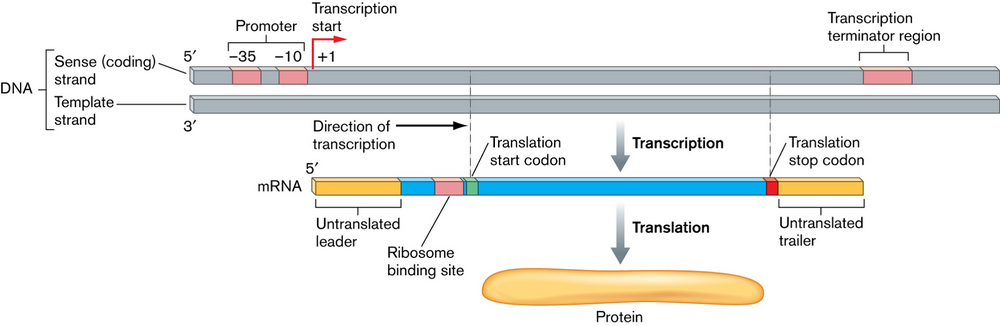
\includegraphics[width=0.99\textwidth]{figs/genes/structure-gene-bacterial.png}
    \caption{A structure of a typical gene.}
    \label{fig:w-gene-structure}
\end{figure*}

Figure~\ref{fig:w-gene-structure} shows a typical gene structure as we have described above. Note that this structure represents a bacterial (prokaryotic) genome, where genes are typically organized without introns. In contrast, in eukaryotic genomes, genes contain introns that are removed during a process called splicing, leaving only exons to form the mature mRNA.

\section{Open Reading Frames}

An {\em open reading frame (ORF)} is a continuous stretch of nucleotides in a DNA sequence that has the potential to be translated into a protein. It begins with a start codon (usually ATG) and extends up to, but does not include, a stop codon (such as TAA, TAG, or TGA), which signals the end of translation. An ORF is different from a {\em reading frame}, which refers to one of the three possible ways in which a nucleotide sequence can be read in sets of three nucleotides (codons). A reading frame becomes an open reading frame only when it includes a start codon, a series of codons that could code for amino acids, and ends with a stop codon, indicating a potential protein-coding sequence. Not all reading frames are open reading frames, as some may not contain both a start and stop codon.

An {\em open reading frame (ORF)} is not necessarily the coding sequence of a gene because the start codon, an {\em ATG}, also encodes the amino acid methionine, which can appear within a gene, not just at the start. This means that an ORF could be part of a larger sequence or occur in non-coding regions where it doesn't correspond to a functional gene. Additionally, regulatory elements and post-transcriptional modifications, like splicing, may result in ORFs that are never translated into functional proteins. Therefore, while ORFs are potential coding sequences, not all ORFs correspond to actual gene-coding regions.


In general, the term ORF can apply to all uninterrupted sequences between a start and stop codon, not necessarily limited to the longest one, as many smaller ORFs may be present within a gene sequence. However, when identifying coding regions, researchers often prioritize the longest ORF as it is more likely to represent the primary protein-coding sequence. For this reason, open reading frame typically refers to the longest possible stretch of DNA (or RNA) between a start codon (often ATG in DNA) and a stop codon (TAA, TAG, or TGA in DNA) that could be translated into a protein. 

\section{Gene Prediction}

{\em Gene prediction} is the process of identifying the location and structure of genes in a genome. This is a crucial step in understanding the genetic information encoded in a genome and is essential for studying gene function, evolution, and disease. Gene prediction can be done using computational methods, which analyze DNA sequences to identify potential genes based on sequence features and patterns.

We will greatly simplify the process of gene prediction here and focus only on finding the longest open reading frames, i.e. the longest stretches between start and any stop codon. Let us start with a Python code that finds all open reading frames in a given DNA sequence.

\vspace*{3mm}
\begin{lstlisting}
from Bio import SeqIO
from Bio.Seq import Seq

def codon_walk(s, frame=0):
    """Walk through a sequence in codons."""
    for ix in range(frame, len(s), 3):
        yield ix, s[ix:ix+3]


def orf_finder(seq, frame, strand=1):
    """Find the longest ORFs in a sequence."""
    orfs = []
    start = None
    n = len(seq)
    for index, codon in codon_walk(seq, frame):
        if not start and codon in START_CODON:
            start = index
        # +3 below for including the stop codon
        elif start and codon in STOP_CODON:
            if strand == 1:
                orfs.append((start, index+3, strand))
            else:
                orfs.append((n-(index+3), n-start, strand))
            start = None
    return orfs

def get_orfs(seq):
    """Get ORFs from a sequence and its reverse complement."""
    orfs = []
    for s, strand in ((seq, 1), (seq.reverse_complement(), -1)):
        for frame in range(3):
            orfs.extend(orf_finder(s, frame, strand))
    return orfs
\end{lstlisting}

The function \texttt{codon\_walk} is a generator that walks through a sequence in codons. The function \texttt{orf\_finder} finds open reading frames in a sequence; it remembers the first occurence of the start codon, and when it hits the stop codon in the current reading frame saves it to the list. The function \texttt{get\_orfs} finds ORFs in a sequence and its reverse complement.

Biologically, the stop codon is not translated and thus not considered part of the ORF, but in our code we include it in the returned sequence so we can easily see which stop codon was encountered and verify correctness.

Let us test the code first using a really short sequence:

\vspace*{3mm}
\begin{lstlisting}
>>> START_CODON = set(["ATG"])
>>> STOP_CODON = set(["TAA", "TAG", "TGA"])
>>> seq = Seq("AAACTAATGTTTTTTATGTTTTAAAAAAACATA")
>>> orfs = get_orfs(seq)
>>> orfs
[(6, 24, 1), (20, 32, -1)]
>>> for start, end, strand in orfs:
...    print(f"ORF: {start}-{end}, {int((end-start)/3) - 1}"
...    "(strand: {strand})")
...    s = seq[start:end] if strand==1 
...        else seq[start:end].reverse_complement()
...    print(f"{s}")
...    print()
...
ORF: 6-24, 5 (strand: 1)
ATGTTTTTTATGTTTTAA

ORF: 20-32, 3 (strand: -1)
ATGTTTTTTTAA
\end{lstlisting}

This looks ok, but let us test the code on a real genome. We will use the genome of {\em Mycoplasma genitalium}, a bacterium with one of the smallest genomes known for a free-living organism. In {\em M. genitalium}, the TGA codon is unusual because it is typically a stop codon in most organisms, but in this organism, it encodes the amino acid tryptophan (Trp) instead of signaling termination. Therefore, the functional stop codons in M. genitalium are only TAA and TAG.

\vspace*{3mm}
\begin{lstlisting}
>>> seq = SeqIO.read("data/m_genitalium.fasta", "fasta").seq
>>> START_CODON = set(["ATG"])
>>> STOP_CODON = set(["TAA", "TAG"])
>>> orfs = get_orfs(seq)
>>> len(orfs)
10716
\end{lstlisting}

That's a lot of open reading frames! {\em M. genetalium}, in fact, has only about 500 protein-coding genes. So not all of these ORFs are actual genes. And then could also miss some of the 

For a start, we can filter out the ORFs that are too short to be considered protein-coding genes. But how long actully are ORFs that we found? And how long are the actual genes in the genome? It is time to find this out.

\section{ORF Lengths}

First, we start with our ORFs. Remember, we already looked for the longest stretches of DNA between start and stop codons, and were therefore already biased towards longer sequences. But how long are they?

\vspace*{3mm}
\begin{lstlisting}
>>> n = len(orfs)
>>> for i in range(0, 200, 20):
>>>     k = sum(1 for l in lengths if i <= l < i+20)
>>>     print(f"{i:3} .. {i+20:3}: {k:>5,} ({k/n:4.1%})")
  0 ..  20: 7,030 (65.6%)
 20 ..  40: 2,036 (19.0%)
 40 ..  60:   639 (6.0%)
 60 ..  80:   262 (2.4%)
 80 .. 100:   136 (1.3%)
100 .. 120:    92 (0.9%)
120 .. 140:    54 (0.5%)
140 .. 160:    41 (0.4%)
160 .. 180:    42 (0.4%)
180 .. 200:    27 (0.3%)
>>> print(f"ORFs longer than {lmax}: {k:,} ({k/n:4.1%})")
ORFs longer than 200: 354 (3.3%)
\end{lstlisting}

The vast majority of our ORFs are short—--too short, in fact, to be considered protein-coding genes. However, there are also some longer ORFs. Filtering out the shorter ones could be beneficial, but what would be a reasonable length threshold to use? Several approaches can help determine this, and we will examine them one at a time.

\section{Permutation Test}

Start and stop codons are not just randomly placed throughout the genome. At least we hope so. :). Throughout the evolution, the genome been reshaped to contain those codon at the right places so that within them the open reading frames are long enough to be considered genes. Surely, therefore, the distribution of the length of ORFs should be different from the ORFs inferred from some random sequence. We can test this hypothesis using a permutation test.

Let's permute our input sequence, and redo the ORF search.

\vspace*{3mm}
\begin{lstlisting}
import random
seq = list(seq)
random.seed(42)
random.shuffle(seq)
seq = Seq("".join(seq))
orfs = get_orfs(seq)

lengths = [int((end-start)/3-1) for start, end, _ in orfs]
report_length_dist(lengths)
\end{lstlisting}

We packed the code that reports on length distribution within \texttt{report\_length\_dist} (not shown here). Running the code, we get:

\vspace*{3mm}
\begin{lstlisting}
  0 ..  20: 11,133 (68.1%)
 20 ..  40: 3,607 (22.1%)
 40 ..  60: 1,153 (7.1%)
 60 ..  80:   301 (1.8%)
 80 .. 100:   104 (0.6%)
100 .. 120:    35 (0.2%)
120 .. 140:     5 (0.0%)
140 .. 160:     1 (0.0%)
160 .. 180:     0 (0.0%)
180 .. 200:     0 (0.0%)
ORFs longer than 200: 0 (0.0%)
\end{lstlisting}

That's a major difference with the distribution of ORF lengths when these are inferred from the actual, non-permuted sequence. In the permuted sequence, there are no ORFs longer than 200 codons, while in the actual sequence, there are 354 of them. This suggests that the distribution of ORF lengths in the actual sequence is not random and that the ORFs we found are not just random stretches of DNA.

We can use this information to set a threshold for the minimum ORF length. For example, we could set the threshold so that there is only a small chance that an ORF of that length would be found in a permuted sequence. Let us denote this probability as $\alpha$. By setting $\alpha = 0.05$, we indicate that we are willing to accept a 5\% probability of incorrectly identifying a random sequence as an ORF of interest. Thus, we would set the minimum ORF length threshold so that only 5\% of ORFs in a randomly permuted sequence would meet or exceed this length:

\vspace*{3mm}
\begin{lstlisting}
>>> alpha = 0.05
>>> sorted(lengths, reverse=True)[int(len(orfs)*alpha)]
50
\end{lstlisting}

Turns out, in our permutation experiment, we need to set the threshold to 50. Setting $\alpha$ to, say, $0.01$, we would be more stringent and accept only 1\% probability of incorrectly identifying a random sequence as an ORF of interest. The threshold would then be:

\vspace*{3mm}
\begin{lstlisting}
>>> alpha = 0.01
>>> sorted(lengths, reverse=True)[int(len(orfs)*alpha)]
77
\end{lstlisting}

Oh, well, it all depends on our choice of the degree of error we are willing to accept. In one way, we have replaced one problem, one parameter, with another, but at least we now think we understand what is going on and know that our threshold should be set probably in the range from 50 to, say, 100.

\section{Mutlinomial Sequence Model}

Another approach to determining the minimum ORF length threshold is to use a multinomial sequence model. This model assumes that the sequence is generated by a distribution where each codon is drawn independently. We can either estimate the actual codon frequencies from the genome, or in a simplified case, assume all codons are equally likely (i.e., an i.i.d. uniform model, which is a special case of a multinomial distribution). Let's proceed with the latter and see where this leads us.

Let us denote the probability of a run of a $k$ or more non-stop codons with $P$, and assert that this probability should be less than $\alpha$, the level of the error we would accept for finding the ORF if the sequence would be random. Assuming all codons are equally likely, and taking into account that there ae (usually) three stop codons, we can write:

$$ P = \left(\frac{61}{64}\right)^k \leq \alpha  $$

It is then easy to solve this equation for $k$:

$$ k \geq \frac{\log(\alpha)}{\log(61) - log(64)} $$

With $\alpha = 0.05$, we get $k\approx 63$, and with $\alpha = 0.01$, we get $k\approx 96$. Which matches well with what we have found using the permutation test. Again, given a specific genome, we could be more precise by estimating the actual codon frequencies.

\section{Comparison with Actual Gene Models}

To find an appropriate threshold for the minimum ORF length, we can also compare the ORFs we identified with the actual gene models in the genome. For this purpose, we can consider an organism that has been well-studied and has an annotated genome, meaning the locations of the genes are known. By comparing the ORFs we found, filtered by length, with the actual genes in the genome, we can evaluate how well they match.

We need two main ingredients for this approach: the annotated genome and criteria to assess how closely our ORFs match the actual genes.

Let us start with the first ingredient. The annotated genomes can be accessed in the public databases, such as NCBI, and the following code will do the work, plus it will save the annotations to the local file for later reuse:

\vspace*{3mm}
\begin{lstlisting}
import os
import pickle
from Bio import Entrez

organism_id = {
    "Hs_21q": "BA000005.3",  # H. sapiens chromosome 21q
    "Mt": "AL123456.3",  # Mycobacterium tuberculosis
    "Mg": "NC_000908.2",  # Mycoplasma genitalium
    "Ec": "NC_000913",  # E coli
}

def load_gene_model(organism):
    filename = f"data/{organism}-gb.pickled"
    if os.path.exists(filename):
        # Load the sequence record from the pickle file
        with open(filename, "rb") as f:
            rec = pickle.load(f)
    else:
        # Fetch the sequence from NCBI if not cached locally
        Entrez.email = "your-email-here"
        with Entrez.efetch(
            db="nucleotide",
            rettype="gbwithparts",
            retmode="text",
            id=organism_id[organism]
        ) as handle:
            rec = SeqIO.read(handle, "gb")
        
        # Save the fetched record to a pickle file for future use
        with open(filename, "wb") as f:
            pickle.dump(rec, f)
    return rec
\end{lstlisting}

Let us load the gene model for {\em M. genitalium} and see what kind of features do we have access to:

\vspace*{3mm}
\begin{lstlisting}
>>> model = load_gene_model("Mg")
>>> model.description
'Mycoplasmoides genitalium G37, complete sequence'
>>> len(model.features)
1137
>>> Counter(f.type for f in model.features)
Counter({'gene': 568,
         'CDS': 526,
         'tRNA': 36,
         'rRNA': 3,
         'ncRNA': 2,
         'source': 1,
         'tmRNA': 1})
\end{lstlisting}

Of the features above, there are two that may interest us. The {\em gene} annotation marks the entire region of DNA that defines a gene, including both coding and non-coding regions necessary for its function, such as regulatory elements, exons, and introns. In contrast, the {\em CDS} (Coding Sequence) annotation specifies only the segment that codes for the protein, starting from the start codon and ending at the stop codon, excluding non-coding regions like introns and regulatory sequences. Thus, while the gene encompasses all parts involved in the expression and regulation of a gene product, the CDS is limited to the exact sequence translated into a protein.

For our comparison with the ORFs we found, we therefore need to consider CDS, the coding sequences. There are 526 of them in the {\em M. genitalium} genome. 

Our second ingredient is the criteria for assessing how well our ORFs match the actual genes. To do this, we can use several scoring functions from the field of machine learning. First, we define the following terms:

\begin{itemize}
    \item \textbf{TP} (True Positives): The number of ORFs correctly identified as genes.
    \item \textbf{FP} (False Positives): The number of ORFs incorrectly identified as genes.
    \item \textbf{FN} (False Negatives): The number of actual genes not identified as ORFs.
    \item \#predictions: The total number of predicted ORFs.
    \item \#genes: The total number of actual genes in the annotated genome.
\end{itemize}

Using these definitions, we can calculate:

\begin{itemize}
    \item \textbf{Precision}: The fraction of correctly identified ORFs among all identified ORFs.
    \[
    \text{Precision} = \frac{\text{TP}}{\text{TP} + \text{FP}}
    \]
    
    \item \textbf{Recall}: The fraction of correctly identified ORFs among all actual genes.
    \[
    \text{Recall} = \frac{\text{TP}}{\text{TP} + \text{FN}}
    \]
    
    \item \textbf{F1 Score}: The harmonic mean of precision and recall, balancing the two.
    \[
    \text{F1 Score} = 2 \cdot \frac{\text{Precision} \times \text{Recall}}{\text{Precision} + \text{Recall}}
    \]
\end{itemize}

Here is now our battle plan: we find all the longest ORFs in the genome, then threshold them by length $L$, and compare them with the actual genes in the genome. We will use the F1 score as our main metric to evaluate how well our ORFs match the actual genes. We will then vary the threshold $L$ and see how the F1 score changes. Below, we assume the \texttt{model} and the sequence \texttt{seq} are aready loaded.

\vspace*{3mm}
\begin{lstlisting}
cds = [f for f in model.features if f.type == "CDS"]
orfs = get_orfs(seq)

locs = set((int(c.location.start), int(c.location.end),
            c.location.strand) for c in cds)

print(f"{'L':>3} {'Pred':>4} {'True':>5} {'False':>5} "
      f"{'Prec':>5} {'Rec':>5} {'F1':>5}")
for min_len in range(50, 200, 10):
    sel = [orf for orf in orfs 
           if ((orf[1] - orf[0]) / 3 - 1) > min_len]

    tp = [strand for (s, e, strand) in sel 
          if (s, e, strand) in locs]
    prec = len(tp) / len(sel)
    recall = len(tp) / len(locs)
    f1 = 2 * prec * recall / (prec + recall)
    print(f"{min_len:3d} {len(sel):4d} {len(tp):4d} "
          f"{len(sel) - len(tp):6d} "
          f"{prec:5.3f} {recall:5.3f} {f1:5.3f}")
\end{lstlisting}

Most of the above code is just for the output formatting. The actual calculation of the F1 score is done in the loop. Note also that we store the actual locations of the genes in the set \texttt{locs} for faster lookup. Running the code, we get:

\vspace*{3mm}
\begin{lstlisting}
    L Pred  True False  Prec   Rec    F1
    50 3172 1466   1706 0.462 0.858 0.601
    60 2524 1453   1071 0.576 0.850 0.687
    70 2142 1432    710 0.669 0.838 0.744
    80 1945 1411    534 0.725 0.826 0.772
    90 1798 1383    415 0.769 0.809 0.789
   100 1679 1342    337 0.799 0.785 0.792
   110 1588 1305    283 0.822 0.764 0.792
   120 1522 1274    248 0.837 0.745 0.789
   130 1469 1241    228 0.845 0.726 0.781
   140 1419 1214    205 0.856 0.710 0.776
   150 1371 1174    197 0.856 0.687 0.762
   160 1323 1135    188 0.858 0.664 0.749
   170 1272 1093    179 0.859 0.640 0.733
   180 1228 1057    171 0.861 0.618 0.720
   190 1182 1015    167 0.859 0.594 0.702
\end{lstlisting}

The F1 score is highest for $L=100$, which is consistent with our previous findings. The F1 score is a good metric for evaluating the performance of our ORF prediction, as it balances precision and recall. In this case, the F1 score is highest when the minimum ORF length threshold is set to 100 codons. This threshold gives us a good balance between correctly identifying ORFs and avoiding false positives.

\section{What's Next?}

Admittedly, identifying genes based solely on ORFs and filtering out spurious ones by length is a simplistic approach, though it serves as a good starting point. In reality, gene prediction is a complex process involving additional steps such as identifying promoter regions, splice sites, and regulatory elements. Furthermore, gene prediction often leverages machine learning models that can learn patterns in the data to make more accurate predictions. Here, however, we will stick with our basic approach and move on to the next chapter, where we will explore methods for comparing gene sequences across and within species.